\documentclass[a4paper]{article}

\makeatletter
\title{Geometria}\let\Title\@title
\author{Andrea Gallese}\let\Author\@author
\date{\today}\let\Date\@date

\usepackage[italian]{babel}
\usepackage[utf8]{inputenc}

\usepackage{mathtools}
\usepackage{amssymb}
\usepackage{amsthm}
\usepackage{faktor}
\usepackage{wasysym}

\usepackage[margin=1.5cm]{geometry}
\usepackage{fancyhdr}
\usepackage{subfig}
\usepackage{multirow}

\usepackage{lipsum}
\usepackage{titlesec}
\usepackage{multicol}
\usepackage{setspace}
\usepackage{mdframed}

\usepackage{color}

% Comando Intitolante
\newcommand{\Intitola}{\begin{center}
		\vspace*{0,5 cm}
		{\Huge \textsc{\Title}} \\
		\vspace{0,5 cm}
		\textsc{\Author} \hspace{1cm} \textsc{\Date}
		\thispagestyle{empty}
		\vspace{0,7 cm}
\end{center}}

% Formato Teoremi, Dimostrazioni, Definizioni
\newtheorem{theorem}{Teorema}[section]
\theoremstyle{remark}
\newtheorem*{remark}{Osservazione}
\theoremstyle{definition}
\newtheorem{definition}[theorem]{Definizione}
\renewcommand\qedsymbol{$\clubsuit$}

% Frontespizio e piè di pagina
\pagestyle{fancy}
\fancyhf{}
\rhead{\textsf{\Author}}
\chead{\textbf{\textsf{\Title}}}
\lhead{\textsf{\today}}

% Per avere le sezioni con le lettere
\renewcommand{\thesection}{\Alph{section}}

%Comandi specifici
\newcommand{\Aut}[1]{\mathrm{Aut}\left( #1 \right)}
\newcommand{\Int}[1]{\mathrm{Int}\left( #1 \right)}
\newcommand{\Orb}[1]{\mathcal{O}rb\left( #1 \right)}
\newcommand{\Stab}[1]{\mathcal{S}tab\left( #1 \right)}

\newcommand{\fun}[5]{\begin{align*}
	#1 \colon #2 &\to #3 \\
	#4 &\mapsto #5
	\end{align*}}

% indentazione
\setlength{\parindent}{0pt}

% multicols
\usepackage{multicol}
\setlength\columnsep{20pt}
\setlength{\columnseprule}{0,5pt}

% Per disegnare diagrammi commuatativi
\usepackage{tikz-cd}

% Serve a decidere il bullet delle liste puntate
\renewcommand\labelitemi{-}

\begin{document}
\Intitola
\small
\begin{multicols}{2}
\begin{center}
	\textsc{Quadrilateri Ciclici}
\end{center}

\textbf{Problema 0.} Quante circonferenze ci trovo nella configurazione delle altezze?. \\

\textbf{Problema 1.} [Feb 13] Abbiamo un quadrilatero i cui lati misurano, nell’ordine, 1, 7, 5, 5. Quanto vale al massimo la sua area? \\

\emph{Soluzione.} Un triangolo con due lati fissati ha area massima quando questi sono fra loro perpendicolari. Fortunatamente \[ 1^2 + 7^2 = 5^2 + 5^2 \]
	
\textsf{I quadrilateri ciclici ci servono a scoprire le circonferenze, che ci permettono di "spostare" gli angoli attraverso una configurazione: è molto importare scovarli e a volte la loro condizione si presenta in modo buffo, è bene conoscerla in tutte le sue forme.} \\

\textbf{Problema 2.} [Feb 2015] Sia $ ABCD $ un quadrilatero convesso tale che $ AB = AC = AD $ e $ BC < CD $. La bisettrice dell’angolo $ B\hat{A}D $ interseca internamente $ CD $ in $ M $ e il prolungamento di $ BC $ in $ N $. Dimostrare che
\begin{itemize}
	\item [(a)] il quadrilatero $ ABCM $ è inscrittibile in una circonferenza;
	\item [(b)] i triangoli $ \bigtriangleup ANB $ e $ \bigtriangleup ABM $ sono simili.
\end{itemize}


\emph{Soluzione.} L'angolo $ B\hat{C}D $ insiste sull'arco minore $ BD $, dunque è l'angolo supplementare di $ B\hat{A}N = B\hat{A}C / 2 $.

\begin{center}
	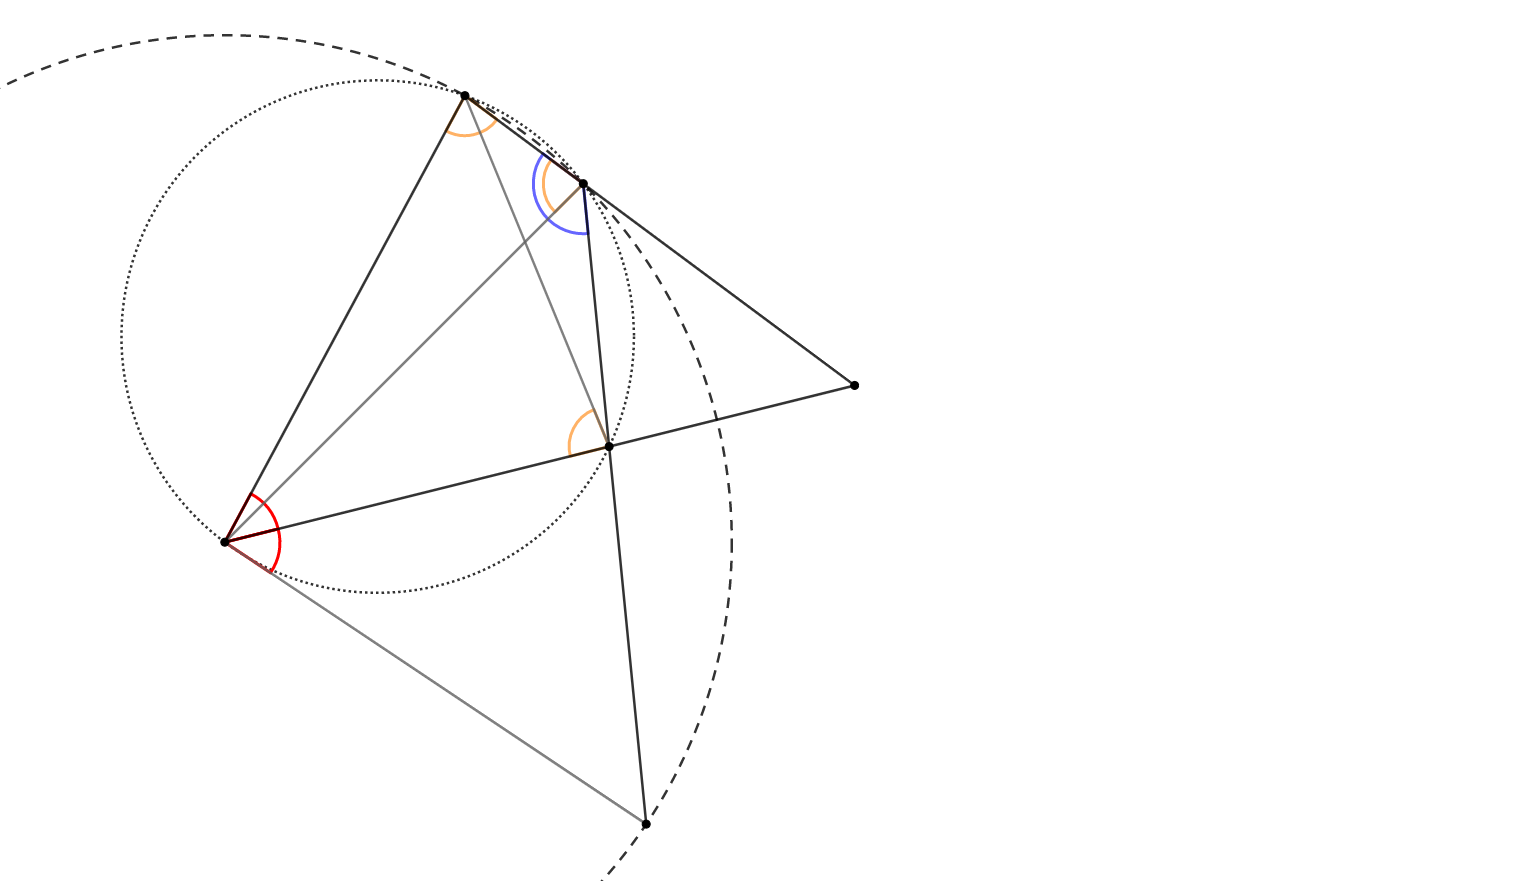
\includegraphics[scale=0.2]{baah}
\end{center}

Grazie, rispettivamente, alla ciclicità appena trovata e al triangolo isoscele $ \bigtriangleup ADB $, si ha
\[ A\hat{N}B = A\hat{C}B = A\hat{B}C.  \]

\textbf{Problema 4.} Sia $ ABC $ un triangolo isoscele su base $ BC $ e siano $ D $, $ E $ punti sui lati $ AB $, $ BC $ rispettivamente,
tali che che le rette $ DE $ e $ AC $ risultino parallele. Si consideri inoltre il punto $ F $ sulla retta $ DE $
che si trova dalla parte opposta di $ D $ rispetto ad $ E $ ed \`e tale che $ F E $ sia congruente ad $ AD $.
Detto $ O $ il circocentro del triangolo $ BDE $, dimostrare che i punti $ O $, $ F $, $ A $, $ D $ giacciono su una
circonferenza.

\columnbreak
\begin{center}
	\textsc{La configurazione Ortocentro-Circocentro}
\end{center}

\begin{center}
	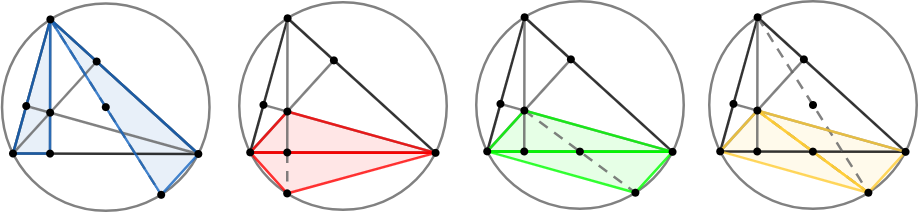
\includegraphics[scale=0.25]{ehiu}
\end{center}

\textbf{Fatto 1.} L'angolo che stacca un'altezza su un lato adiacente è uguale all'angolo che stacca il raggio uscente dallo stesso vertice sull'altro lato che esce da quel vertice. \\

\textbf{Fatto 2.} Il simmetrico dell'ortocentro rispetto a un lato giace sulla circonferenza circoscritta al triangolo. \\

\textbf{Fatto 3.} Il simmetrico dell'ortocentro rispetto al punto medio di un lato giace sulla circonferenza circoscritta al triangolo. \\

\textbf{Fatto 4.} Il simmetrico dell'ortocentro rispetto a un lato è il punto diametralmente opposto al vertice che non appartiene al lato di riflessione. \\

\textcolor{gray}{\textbf{Fatto 5.} L'ortocentro è l'incentro del triangolo ortico. O meglio, i lati del triangolo ortico staccano angoli uguali sul lato.} \\

\iffalse
\begin{center}
	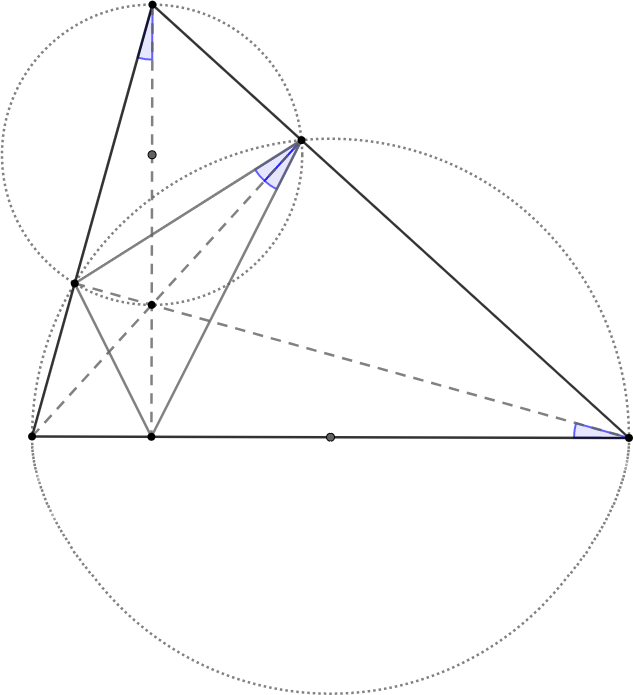
\includegraphics[scale=0.20]{cosa5}
\end{center}
\fi

\textcolor{gray}{\textbf{Fatto 6.} I triangoli adiacenti all'ortico sono tutti simili a quello di partenza.} \\

\textbf{Problema 3.} [Feb 17] Data una circonferenza $ \omega $ di diametro $ AB $ e $ P $ un punto interno al segmento $ AB $, sia $ M $ il punto medio di $ PB $. Siano $ r $, $ s $ due rette parallele passanti rispettivamente per $ M $, $ P $, non coincidenti con la retta $ AB $ nè ad essa ortogonali. Sia poi $ H $ la proiezione ortogonale di $ A $ su $ s $ e sia $ K $ il punto d’intersezione (distinto da $ A $) tra $ \omega $ e la retta $ AH $. Siano infine $ X $, $ Y $ le intersezioni di $ r $ con $ \omega $, dove $ X $ è dalla parte opposta di $ H $ rispetto ad $ AB $.
\begin{itemize}
	\item [(a)] Dimostrare che il triangolo $ \bigtriangleup HYK $ è isoscele.
	\item [(b)] Dimostrare che $ BXHY $ è un parallelogramma.
\end{itemize}
 
 %\iffalse
 \begin{center}
 	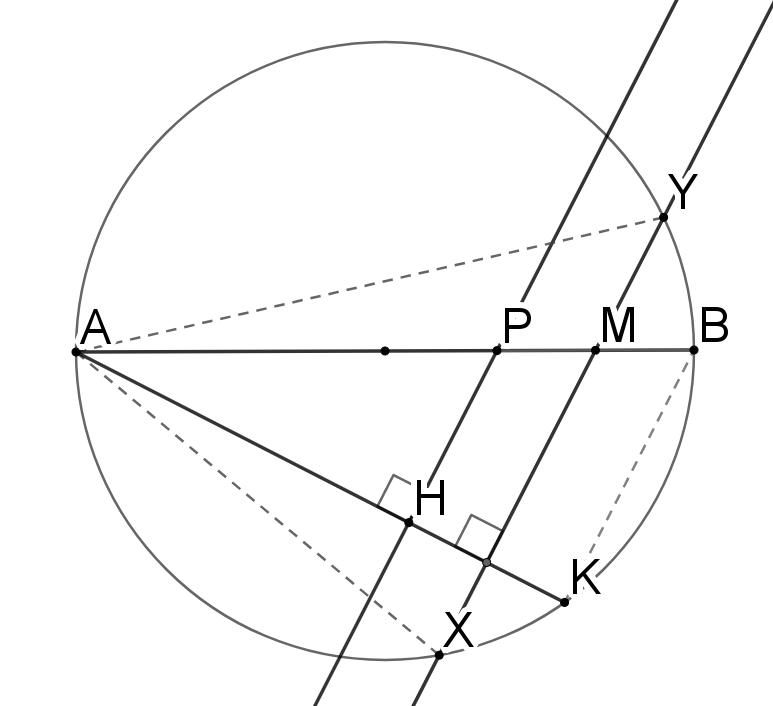
\includegraphics[scale=0.20]{Febb17}
 \end{center}
 %\fi
 
 \textsf{Probabilmente conoscono il problema, è interessante interpretarlo in funzione dei fatti noti!}


\columnbreak
\vspace{0.5 cm}
\begin{center}
	\textsc{La configurazione delle bisettrici}
\end{center}

%\iffalse
\begin{center}
	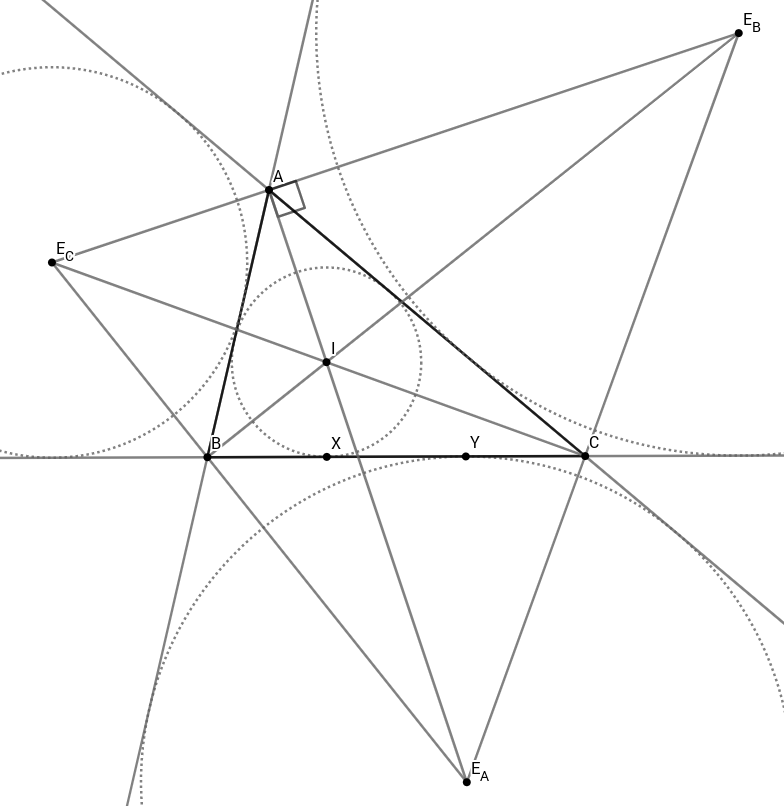
\includegraphics[scale=0.20]{nmode}
\end{center}
%\fi


\textbf{Fatto 1.} Bisettrice interna ed esterna sono perpendicolari. \\

\textbf{Fatto 2.} Le bisettrici concorrono a tre a tre. \\

\textbf{Fatto 3.} I punti in cui concorrono le bisettrici estere sono centri delle circonferenze tangenti esternamente ai lati. \\

\textbf{Fatto 4.} Il punto medio tra incentro ed excentro giace sulla circoscritta. \\

\textcolor{gray}{\textbf{Fatto 5.} Il triangolo di partenza è l'ortico del triangolo degli excentri. \\
} % si riesce a sfruttare questo fatto per mostrare che i punti medi tra otrocentro e vertice giacciono sulla circonferenza di Feuerbach

\textcolor{gray}{\textbf{Fatto 6.} Il lati del pedale dell'incentro sono perpendicolari alle bisettrici.  \\
}

\end{multicols}

\begin{center}
	\textsc{Trasformazioni del piano}
\end{center}
\begin{multicols}{2}

\begin{center}
	\textsc{Riflessione.}
\end{center}

\textbf{Problema 0.} Cappuccetto Rosso.\\

\textbf{Fatto 1.} Proprietà ottica dell'ellisse. \\ 

\textbf{Problema 1.} Il traghettatore. \\

\textbf{Fatto 2.} Simmetrici di ortocentro sulla circoscritta. \\

\begin{center}
	\textsc{Traslazione.}
\end{center}

\textbf{Fatto 3.} Le traslazioni provocano parallelogrammi.\\

\textbf{Problema 3.} The opposite sides of a
hexagon ABCDEF are parallel. If
$$  BC-EF = ED-AB = AF-CD > 0  $$ show
that all angles of $ ABCDEF $ are equal. \\

\begin{center}
	\textsc{Rotazione.}
\end{center}

\textbf{Fatto 4.} Le rotazioni mi formano angoli incidenti noti.\\

\textbf{Problema 4.} $ ABCD $ is a unit square.
Points $ P,\, Q,\, M,\, N $ are on sides $ AB,\, BC,\,
CD,\, DA $ respectively such that
$$  AP + AN + CQ + CM = 2  $$
Prove that $ PM \perp QN $. \\

\textbf{Problema 5.} Sul segmento $ AB $ scegliamo un punto $ C $, costruiamo poi i quadrati $ ACDE $ e $ CBFG $, dallo stesso lato. Mostrare che $ AG $ e $ BD $ si intersecano nel punto di intersezione delle circoscritte ai due quadrati.\\

\end{multicols}

\newpage
\begin{center}
	\textsc{Potenza di un punto rispetto a una circonferenza}
\end{center}
\begin{multicols}{2}
	
	Ripasso sulle circonferenze \\
	
	\textbf{Problema 0.} Configurazione delle altezze. \\
	
	\textbf{Problema 4.} Let $ C_1, C_2, C_3, C_4 $ be four distinct circles. For $ i = 1, 2, 3, 4 $,
	suppose that $ C_i  $ and $ C_{i+1}  $ intersect at two distinct points $ A_i $ and $ B_i $ (here $ C_5 = C_1 $). Prove that if $ A_1A_2A_3A_4 $ is cyclic then so is $ B_1B_2B_3B_4 $. \textsf{(nella versione semplificata in cui scegliamo il quadrilatero ciclico)} \\
	
	I teoremi delle secanti, delle corde e delle tangenti. \\
	
	\textbf{Definizione.} Prendiamo da $ P $ una secante a caso, diciamo che interseca $ \omega $ in A e B, allora 
	\[ \text{Pow}_{\omega}(P) = PA \cdot PB \]
	
	\textcolor{gray}{\textbf{Fatto 4.} $ OI^2 = R(R-2r) $} \\
	
	\textbf{Teorema 1.} Let $ A,\, B,\, C,\, D $ be four distinct points. Let lines $ AB $
	and $ CD $ intersect at $ P $. Assume that either
	\begin{enumerate}
		\item $ P $ lies on both line segments $ AB $ and $ CD $, or
		\item $ P $ lies on neither line segments.
	\end{enumerate}
	Then $ A,\, B,\, C,\, D $ are concyclic if and only if $ PA\cdot PB  = PC\cdot PD$. \\
	
	\textbf{Problema 1.} Let ABC be an acute triangle. Let the line through B perpendicular to AC meet the
	circle with diameter AC at points P and Q, and let the line through C perpendicular
	to AB meet the circle with diameter AB at points R and S. Prove that P, Q, R, S are
	concyclic. \\
	
	\textcolor{gray}{\textbf{Fatto 1.} Esistenza della circonferenza dei nove punti.} \\
	
	\textcolor{gray}{\textbf{Problema 2.} $ M $ è il punto medio del lato $ AC $ di un triangolo $ \bigtriangleup ABC $. $ P $ e $ Q $ sono punti interni, rispettivamente, ad $ AM $ e $ CM $ tali che $ PQ =  AC/2 $. La circonferenza passante per $ A,\,B $
	e $ Q $ interseca $ BC $ in $ X $ e la circonferenza passante per $ B,\,C $ e $ P $ interseca $ BA $ in
	$ Y $. Provare che il quadrilatero $ BXMY $ è ciclico.} \\

	\textbf{Definizione.} di Asse radicale. L'asse è una retta perpendicolare alla retta dei centri. \\
	
	\textbf{Problema 3.} Let $ \Gamma_1 $ and $ \Gamma_2 $ be two intersecting circles. Let a common tangent to $ \Gamma_1 $ and $ \Gamma_2 $ touch $ \Gamma_1 $
	at $ A $ and $ \Gamma_2 $ at $ B $. Show that the common chord of $ \Gamma_1 $ and $ \Gamma_2 $, when extended, bisects
	segment $ AB $. \\
	
	\textbf{Teorema 2.} Concorrenza degli assi radicali \\
	
	\textbf{Fatto 2.} Gli assi concorrono. \\
	
	\textbf{Fatto 3.} Le altezze concorrono. \\
	
	\textcolor{gray}{\textbf{Problema 4.} Let $ A,\, B,\, C $, and $ D $ be four distinct points on a line, in that order. The
	circles with diameters $ AC $ and $ BD $ intersect at $ X $ and $ Y $ . The line $ XY $ meets $ BC $ at $ Z $.
	Let $ P $ be a point on the line $ XY $ other than $ Z $. The line $ CP $ intersects the circle with
	diameter $ AC $ at $ C $ and $ M $, and the line $ BP $ intersects the circle with diameter $ BD $ at $ B $
	and $ N $. Prove that the lines $ AM $, $ DN $, and $ XY $ are concurrent.} \\
	
	\textbf{Problema 5.} Sono date tre circonferenze $ \Gamma $, $ \Gamma_1 $, $ \Gamma_2 $ di raggi rispettivamente 6, 3, 2. $ \Gamma_1 $ e $ \Gamma_2 $ sono tangenti
	esternamente in A, mentre $ \Gamma $ tange entrambe le altre circonferenze internamente, rispettivamente
	in $ A_1 $ ed $ A_2 $ . Determinare il raggio della circonferenza circoscritta ad $ AA_1A_2  $.
	
\end{multicols}


\newpage
\textbf{Problemi.}

\begin{enumerate}

% Senza Tolomeo è rognosetto.
\item (Febbraio 2015.)  Sia $ ABCD $ un quadrilatero tale che $ AB = 24 $, $ BC = 20 $, $ CD = 15 $, $ DA = 7 $, $ BD = 25 $. Quanto è lungo $ AC $?

\item (Febbraio 2012b.) In un triangolo acutangolo $ \bigtriangleup ABC $ con $ AB < AC $, la bisettrice che parte da $ A $ interseca il lato $ BC $ nel punto $ P $. La parallela al lato $ AB $ passante per $ P $ interseca il lato $ AC $ nel punto $ Q $; su questa retta sia $ R $ il punto che giace sulla semiretta uscente da $ Q $ che non contiene $ P $ e tale che $ QR = QA $. Chiamiamo poi $ S $ la proiezione ortogonale di $ R $ su $ BC $ e $ T $ l’intersezione tra $ AC $ e la retta passante per $ P $ e perpendicolare ad $ AP $.
\begin{itemize}
	\item [(a)] Dimostrare che il circocentro di $ \bigtriangleup APR $ è $ Q $;
	\item [(b)] Dimostrare che $ \triangle STC $ è simile ad $ \triangle APC $. 
\end{itemize}

\item  Sia $ AB $ una corda di una circonferenza e $ P $ un punto interno ad $ AB $ tale che $ AP = 2PB $. Sia $ DE $ la corda passante per $ P $ e perpendicolare ad $ AB $. Dimostrare che il punto medio $ Q $ di $ AP $ è l’ortocentro di $ \bigtriangleup ADE $. [Feb 08.]

\item (Febbraio 2010) La casa di Dante si trova nel punto $ D $ ai piedi di una montagna conica con il diametro di base di $ 4 km $ e cima nel punto $ C $. Si sa che $ D $ dista da $ C $ $ 4 km $ in linea retta e che, detto $ P $ il punto diametralmente opposto a $ D $ rispetto alla base della montagna, la porta dell’Inferno si trova a $ 3/4 $ del segmento $ CP $, più vicino a $ P $. Quale distanza deve percorrere Dante al minimo (camminando sulle pendici della montagna) per poter raggiungere la porta dell’Inferno da casa sua?

\item Let $ M $ and $ N $ be the midpoints of sides $ AD $ and $ BC $ of
quadrilateral $ ABCD $ respectively. If
$  2MN = AB+CD,  $
then prove that $ AB\parallel CD $.

\item Inside an equilateral
triangle $ \triangle ABC $, there is a point $ P $ such
that $ PC=3 $, $ PA=4 $ and $ PB=5 $. Find the
perimeter of ABC.

% Bello! Basta un minimo diAngle Chasing.
\item  Let $ \triangle ABC $ be a triangle, and $ P $ a point on its circumcircle. Show that the reflections of $ P $ across the three sides of $ \triangle ABC $ lie on a lie that passes through the orthocenter of $ \triangle ABC $.

\item (Febbraio 2012.) Sia $\triangle ABC $ un triangolo acutangolo; sia $ O $ il suo circocentro e siano $ P $, $ Q $ i punti (diversi da $ A $) in cui rispettivamente l’altezza uscente dal vertice $ A $ e il prolungamento di $ AO $ incontrano la circonferenza circoscritta ad $ \triangle ABC $.
\begin{itemize}
	\item [(a)] Si dimostri che gli angoli $ B\hat{A}P $ e $ Q\hat{A}C $ sono congruenti;
	\item [(b)] Si dimostri che i triangoli $ \triangle BCP $ e $ \triangle CBQ $ sono congruenti;
	\item [(c)] Si dimostri che, detti $ M $ e $ N $ i punti medi di $ AB $ e $ AC $, l’area del quadrilatero $ ABPC $ vale quattro volte l’area del quadrilatero $ AMON $.
\end{itemize}

\item (Febbraio 2010.) È dato un triangolo acutangolo isoscele $ \triangle ABC $ di base $ AC $. All’interno di tale triangolo sono dati un punto $ M $ , dalla parte di $ C $ rispetto all’asse di $ AC $ e tale che $ C\hat{M}A = 2 C\hat{B}A $, e un punto $ N  $ all’interno del segmento $ AM $ tale che $ B\hat{N}M = C\hat{B}A $
\begin{itemize}
	\item [(a)] Dimostrare che $ C\hat{B}N = B\hat{A}M  $.
	\item [(b)] Dimostrare che $ CM + MN = BN $. 
\end{itemize}

% Non si capisce bene cosa si usa.
\item (Febbraio 2017.) Sia $ \triangle ABC $ un triangolo acutangolo e sia $ D $ il piede della bisettrice uscente da $ A $. Sia $ \omega $ la circonferenza per $ A $ tangente a $ BC $ in $ D $, e siano $ E,\, F $ le intersezioni di $ \omega $ con $ AB $, $ AC $ rispettivamente. Le tangenti a $ \omega $ in $ E $ e $ F $ si intersecano in $ P $. Sapendo che $ PE = 3$ e che il raggio di $ \omega $ è 4, quanto misura il segmento $PD$? 

% Si riesce a dimostrare usando la configurazione delle bisettrici!
\item Sia $\triangle ABC $ un triangolo acutangolo e $ D $, $ E $, $ F $ i piedi delle altezze. Chiamato $ X $ il punto medio tra l'ortocentro di $ \triangle ABC $ e $ D $, dimostrare che $ X $ giace sulla circonferenza circoscritta a $\triangle DEF $.

% Facile per un IMO, c'è solo da mostrare che AFQP è ciclico.
\item (Shortlist 2010/G1). Let $ \triangle ABC $ be an acute triangle with $ D,\, E,\, F $ the feet
of the altitudes lying on $ BC,\, CA,\, AB $ respectively. One of the intersection points of the
line $ EF $ and the circumcircle is $ P $. The lines $ BP $ and $ DF $ meet at point $ Q $. Prove that
$ AP = AQ $.

% Carino, ma si formalizza per bene solo con gli angoli orientati.
\item (Folklore). Let $ C_1, C_2, C_3, C_4 $ be four distinct circles. For $ i = 1, 2, 3, 4 $,
suppose that $ C_i  $ and $ C_{i+1}  $ intersect at two distinct points $ A_i $ and $ B_i $ (here $ C_5 = C_1 $). Prove that if $ A_1A_2A_3A_4 $ is cyclic then so is $ B_1B_2B_3B_4 $.

% Molto bello! Usa un sacco di fatti sul pedaqle dell'incentro.
\item In triangle $ \triangle ABC $, let $ D \in  BC ,\, E \in  AC,\, F  \in  AB$ be the points of tangency of the
incircle to the sides. Let $ I $ be the incenter. The parallel line through $ A $ to $ BC $ intersects
$ DE $ and $ DF $ at $ M $ and $ N $, respectively. Let $ L $ and $ T $ be the midpoints of the segments
$ ND $ and $ DM $. Show that $ A,\, L,\, I,\, T $ lie on a circle.

\item (GaS 17 - Semifinale: Strumenti di tortura.)
Discutendo di religione, uno dei matematici si mise a descrivere un complicato strumento di tortura dell’inquisizione
spagnola: partendo da un cubo di lato 568mm, su ogni faccia viene incollata una piramide a base quadrata -coincidente
con la faccia del cubo- e le cui facce laterali sono triangoli equilateri. “Ma è orribile!” disse inorridito un altro “Però ha
una forma davvero interessante, mi chiedo quanto sia lungo in millimetri il percorso minimo che unisce due vertici opposti
qualunque del solido muovendosi sulla sola superficie...” Nota: due vertici si dicono oppostii se sono simmetrici rispetto al
centro del cubo.

\item (GaS 17 - Finale: Il traghettatore.) 
Io e Cartesio giungemmo in fronte a Carnote, il traghettatore. Ei ci venne incontro sulla sua zattera a forma di quadrilatero
convesso $ ABCD $. Essa aveva una forma peculiare: i suoi angoli erano tali che $ A\hat{B}C = A\hat{D}C + B\hat{A}C + B\hat{C}A $ e
$ D\hat{C}A = 2B\hat{A}C $. Inoltre, si aveva $ AC = 91 $, $ AD + CD = 169 $. Ci ordinò di sederci all’interno del triangolo $ \triangle ABC $,
piuttosto stretto, di area 2184. Qual era invece l’area totale della zattera che doveva condurci al di là del fiume
Archimeronte?

\item (GaS 17 - Finale: Tra i fuochi ardenti.) 
Tra gl’iracondi, nei pressi del fiume Stage, sedeva un’altra anima prava, colpevole in vita di non saper controllare la sua
favella. Abile cultore della geometria, anche la più complessa, fu condannato a sedere in mezzo a un esagono $ ABCDEF $
di area 1000, fatto di carboni rossi e roventi. Attorno ad esso ardevano fiamme in forma di sei ellissi, tutte uguali tra loro,
ognuna avente per fuochi due vertici dell’esagono ch’erano adiacenti (estremi dello stesso lato). Quella di fuochi $ A $ e $ B $
era tangente a quella di fuochi $ C $ e $ D $; quella di fuochi $ B $ e $ C $ era tangente a quella di fuochi $ D $ ed $ E $, e così via, in
cerchio. Tutti questi punti di tangenza formavano un poligono; qual era la sua area?

\item (SNS 2011)
Siano $ n, m \geq 2 $ interi e siano $ A_1 , \dots, A_n $ e $ B_1 , \dots , B_m $ due famiglie di punti nel piano tali che $ \overline{A_iB_j} = i + j $ per ogni $ (i, j) $. Si provi che esistono due rette perpendicolari $ a $ e $ b $ tali che tutti gli $ A_i $ giacciono su $ a $ e tutti i $ B_i $ giacciono su $ b $.

\item (Feb 16) Dato un triangolo $ ABC $ di lati $ AB = 13 $, $ BC = 14 $ e $ AC = 15 $, sia $ H $ il piede dell’altezza relativa al lato $ BC $, $ M $ il punto medio di $ BC $ e $ N $ il punto medio di $ AM $. Quanto vale la lunghezza di $ HN $?

\end{enumerate}

% Lo metto qua solo per sbaglio
\textbf{Bellissimo!} In acute triangle $ \triangle ABC $, let $ D,\, E,\, F $ denote the feet of the altitudes from
$ A,\, B,\, C $, respectively, and let $ \omega $ be the circumcircle of $\triangle AEF $. Let $ \omega_1 $ and $ \omega_2 $ be the circles through $ D $ tangent to $ \omega $ at $ E $ and $ F $, respectively. Show that $ \omega_1 $ and $ \omega_2 $ meet at a point $ P $ on $ BC $ other than $ D $.


\newgeometry{left=3cm,bottom=0.1cm}
\begin{center}
	\vspace*{0,5 cm}
	{\Huge \textsc{Geometria - Stage Sassari}} \\
	\vspace{0,5 cm}
	\textsc{\Author} \hspace{1cm} \textsc{14 dicembre 2017}
	\thispagestyle{empty}
	\vspace{0,7 cm}
\end{center}
\normalsize



\begin{enumerate}
	\item  Sia $ ABCD $ un quadrilatero tale che $ AB = 24 $, $ BC = 20 $, $ CD = 15 $, $ DA = 7 $, $ BD = 25 $. Quanto è lungo $ AC $? [Feb 15] 
	
	\item  In un triangolo acutangolo $ \bigtriangleup ABC $ con $ AB < AC $, la bisettrice che parte da $ A $ interseca il lato $ BC $ nel punto $ P $. La parallela al lato $ AB $ passante per $ P $ interseca il lato $ AC $ nel punto $ Q $; su questa retta sia $ R $ il punto che giace sulla semiretta uscente da $ Q $ che non contiene $ P $ e tale che $ QR = QA $. Chiamiamo poi $ S $ la proiezione ortogonale di R su BC e T l’intersezione tra AC e la
	retta passante per $ P $ e perpendicolare ad $ AP $.
	\begin{itemize}
		\item [(a)] Dimostrare che il circocentro di $ \bigtriangleup APR $ è $ Q $;
		\item [(b)] Dimostrare che $ \bigtriangleup STC $ è simile ad $ \bigtriangleup APC $. [Feb 12b]
	\end{itemize}
	
	\item  Sia $ AB $ una corda di una circonferenza e $ P $ un punto interno ad $ AB $ tale che $ AP = 2PB $. Sia $ DE $ la corda passante per $ P $ e perpendicolare ad $ AB $. Dimostrare che il punto medio $ Q $ di $ AP $ è l’ortocentro di $ \bigtriangleup ADE $. [Feb 08.]
	
	\item La casa di Dante si trova nel punto $ D $ ai piedi di una montagna conica con il diametro di base di $ 4 km $ e cima nel punto $ C $. Si sa che $ D $ dista da $ C $ $ 4 km $ in linea retta e che, detto $ P $ il punto diametralmente opposto a $ D $ rispetto alla base della montagna, la porta dell’Inferno si trova a $ 3/4 $ del segmento $ CP $, più vicino a $ P  $. Quale distanza deve percorrere Dante al minimo (camminando sulle pendici della montagna) per poter raggiungere la porta dell’Inferno da casa sua? [Feb 10]
	
	\item Siano $ M $ e $ N $ i punti medi, rispettivamente, dei lati $ AD $ e $ BC $ di un quadrilatero $ ABCD $. Dimostra che, se $ 2MN = AB + CD $, allora $ AB $ è parallelo a $ CD $.
	
	\item In un triangolo equilatero $ \bigtriangleup ABC $, c'è un punto $ P $ tale che $ PC = 3 $, $ PA = 4 $ e $ PB = 5 $. Trova il perimetro di $ \bigtriangleup ABC $.
\end{enumerate}

\newpage
\begin{center}
	\vspace*{0,5 cm}
	{\Huge \textsc{Geometria}} \\
	\vspace{0,5 cm}
	\textsc{\Author} \hspace{1cm} \textsc{5 febbraio 2018 - Massa}
	\thispagestyle{empty}
	\vspace{0,7 cm}
\end{center}
\normalsize

\begin{enumerate}
	% Ciclici + Tolomeo.
	\item (Febbraio 2015).  Sia $ ABCD $ un quadrilatero tale che $$  AB = 24 ,\; BC = 20 ,\; CD = 15 ,\; DA = 7 ,\; BD = 25 . $$ Quanto è lungo $ AC $? 
	
	% Problemino sulla configurazion ortocentro
	\item (Febbraio 2008). Sia $ AB $ una corda di una circonferenza e $ P $ un punto interno ad $ AB $ tale che $ AP = 2PB $. Sia $ DE $ la corda passante per $ P $ e perpendicolare ad $ AB $. Dimostrare che il punto medio $ Q $ di $ AP $ è l’ortocentro di $ \bigtriangleup ADE $. 
	
	% Ciclicità.
	\item (Shortlist 2010/G1). Sia $\bigtriangleup ABC $ un triangolo acutangolo con $ D $, $ E $, $ F $ i piedi delle altezze che giacciono sui lati $ BC $, $ CA $, $ AB $, rispettivamente. Uno dei punti di intersezione tra la retta $ EF $ e la circoscritta è $ P $. Le rette $ BP $ e $ DF $ si incontrano in un punto $ Q $. Dimostra che $ AP = AQ $.
	
	% Configurazione con ortocentro e bisettrici!
	\item (Feuerbach). Sia $ \bigtriangleup ABC $ un triangolo acutangolo e $ D $, $ E $, $ F $ i piedi delle altezze. Chiamato $ X $ il punto medio tra l'ortocentro di $\bigtriangleup ABC $ e $ A $, dimostrare che $ X $ giace sulla circonferenza circoscritta al triangolo $\bigtriangleup DEF $.
	
	
\end{enumerate}

\newpage
\begin{center}
	\vspace*{0,5 cm}
	{\Huge \textsc{Geometria}} \\
	\vspace{0,5 cm}
	\textsc{\Author} \hspace{1cm} \textsc{23 luglio 2018 - Palermo}
	\thispagestyle{empty}
	\vspace{0,7 cm}
\end{center}
\normalsize

\begin{enumerate}
	
	\item Sia $ P $ un punto interno alla base $ AB $ di un triangolo isoscele $ ABC $. Dimostrare che
	\[ PC^2 = AC^2 - AP \cdot BP \]
	
	\item Siano $ A,\, B,\, C $ tre punti su un cerchio $ \Gamma $ tali che $ AB = BC $. Sia $ D $ il punto d'incontro tra le tangenti in $ A $ e in $ B $. $ DC $ interseca nuovamente $ \Gamma $ in $ E $. Dimostra che la retta $ AE $ biseca il segmento $ BD $. \\
	
	\item Sia $ \bigtriangleup ABC $ un triangolo acutangolo con ortocentro $ H $. I punti $ M $ ed $ N $ sono scelti, rispettivamente, sui lati $ AB $ e $ AC $. I cerchi con diametri $ BN $ e $ CM $ si intersecano nei punti $ P $ e $ Q $. Dimostra che $ P $, $ Q $, e $ H $ sono allineati. \\
	
	\item Siano $ n, m \geq 2 $ interi e siano $ A_1 , \dots, A_n $ e $ B_1 , \dots , B_m $ due famiglie di punti nel piano tali che $ {A_iB_j} = \sqrt{i + j} $ per ogni $ (i, j) $. Si provi che esistono due rette perpendicolari $ a $ e $ b $ tali che tutti gli $ A_i $ giacciono su $ a $ e tutti i $ B_i $ giacciono su $ b $. \\
	
	\item Siano $ \mathcal{C}_1 $ and $ \mathcal{C}_2 $ cerchi concentrici, con $ \mathcal{C}_2 $ all'interno di $ \mathcal{C}_1 $. Siano $ A $ un punto di $ \mathcal{C}_1 $ e B un punto di $ \mathcal{C}_2 $ tali che $ AB $ sia tangente a $ \mathcal{C}_2 $. Sia C il secondo punti d'intersezione di $ AB $ con $ \mathcal{C}_1 $, e sia $ D $ il punto medio del segmento $ AB $. Un retta per $ A $ interseca $ \mathcal{C}_2 $ in $ E $ ed $ F $ in modo che gli assi di $ DE $
	e $ CF $ si intersechino in un punto $ M $ su $ AB $. Trova il rapporto $ AM/MC $. \\
	
	\item In un triangolo acutangolo $ \triangle ABC $, denotiamo con $ D,\, E,\, F $ i piedi delle altezze da $ A,\, B,\, C $, rispettivamente, e sia $ \omega $ la circonferenza circoscritta ad $\triangle AEF $. Siano $ \omega_1 $ e $ \omega_2 $ i cerchi passanti per $ D $ tangenti a $ \omega $ in $ E $ ed $ F $, rispettivamente. Dimostra che $ \omega_1 $ e $ \omega_2 $ si incontrano in punto $ P $ su $ BC $ diverso da $ D $. \\
	
\end{enumerate}

\newpage
\begin{center}
	\vspace*{0,5 cm}
	{\Huge \textsc{Geometria}} \\
	\vspace{0,5 cm}
	\textsc{3 febbraio 2019 - Terni}
	\thispagestyle{empty}
	\vspace{0,7 cm}
\end{center}
\normalsize

\begin{enumerate}
	
	\item  (GaS 2017). Giunti finalmente a destinazione, i nostri pellegrini trovarono la tomba di Archimede, sulla cui lapide era inciso un eptagono
	regolare $ ABCDEFG $ di centro $ O $. Con grande disappunto videro che l’incisione era stata vandalizzata con alcune righe:
	il vandalo aveva preso il punto $ X $ simmetrico di $ D $ rispetto alla retta $ BG $, poi aveva intersecato le rette $ XB  $ e $ GO $ in $ Y $.
	Tuttavia osservarono che l’angolo convesso $ C\hat{Y}G $ aveva un valore interessante se espresso in gradi. Quant’è tale numero?
	
	\item Sia $ \bigtriangleup ABC $ un triangolo acutangolo con ortocentro $ H $. I punti $ M $ ed $ N $ sono scelti, rispettivamente, sui lati $ AB $ e $ AC $. I cerchi con diametri $ BN $ e $ CM $ si intersecano nei punti $ P $ e $ Q $. Dimostra che $ P $, $ Q $, e $ H $ sono allineati. \\
	
	% Ciclici + Tolomeo.
	\item (Febbraio 2015).  Sia $ ABCD $ un quadrilatero tale che $$  AB = 24 ,\; BC = 20 ,\; CD = 15 ,\; DA = 7 ,\; BD = 25 . $$ Quanto è lungo $ AC $? 
	
	\item Siano $ A,\, B,\, C $ tre punti su un cerchio $ \Gamma $ tali che $ AB = BC $. Sia $ D $ il punto d'incontro tra le tangenti in $ A $ e in $ B $. $ DC $ interseca nuovamente $ \Gamma $ in $ E $. Dimostra che la retta $ AE $ biseca il segmento $ BD $. \\
	
	\item[$ \star. $] Siano $ \mathcal{C}_1 $ and $ \mathcal{C}_2 $ cerchi concentrici, con $ \mathcal{C}_2 $ all'interno di $ \mathcal{C}_1 $. Siano $ A $ un punto di $ \mathcal{C}_1 $ e B un punto di $ \mathcal{C}_2 $ tali che $ AB $ sia tangente a $ \mathcal{C}_2 $. Sia C il secondo punti d'intersezione di $ AB $ con $ \mathcal{C}_1 $, e sia $ D $ il punto medio del segmento $ AB $. Un retta per $ A $ interseca $ \mathcal{C}_2 $ in $ E $ ed $ F $ in modo che gli assi di $ DE $
	e $ CF $ si intersechino in un punto $ M $ su $ AB $. Trova il rapporto $ AM/MC $. \\
	
	
\end{enumerate}

\newpage
\begin{center}
	\vspace*{0,5 cm}
	{\Huge \textsc{Geometria}} \\
	\vspace{0,5 cm}
	\textsc{Dicembre 2019 - Pavia}
	\thispagestyle{empty}
	\vspace{0,7 cm}
\end{center}
\normalsize

\begin{enumerate}
	% Ciclici + Tolomeo.
	\item (Febbraio 2015).  Sia $ ABCD $ un quadrilatero tale che $$  AB = 24 ,\; BC = 20 ,\; CD = 15 ,\; DA = 7 ,\; BD = 25 . $$ Quanto è lungo $ AC $? 
	
	
	% Problemino sulla configurazion ortocentro
	\item (Febbraio 2008). Sia $ AB $ una corda di una circonferenza e $ P $ un punto interno ad $ AB $ tale che $ AP = 2PB $. Sia $ DE $ la corda passante per $ P $ e perpendicolare ad $ AB $. Dimostrare che il punto medio $ Q $ di $ AP $ è l’ortocentro di $ \bigtriangleup ADE $.
	
	% Ciclicità. Sembra esageratamente difficile, ma forse non vedo le cose.
	\item (Shortlist 2010/G1). Sia $\bigtriangleup ABC $ un triangolo acutangolo con $ D $, $ E $, $ F $ i piedi delle altezze che giacciono sui lati $ BC $, $ CA $, $ AB $, rispettivamente. Uno dei punti di intersezione tra la retta $ EF $ e la circoscritta è $ P $. Le rette $ BP $ e $ DF $ si incontrano in un punto $ Q $. Dimostra che $ AP = AQ $.
	
	% Configurazione con ortocentro e bisettrici!
	\item (Feuerbach). Sia $ \bigtriangleup ABC $ un triangolo acutangolo e $ D $, $ E $, $ F $ i piedi delle altezze. Chiamato $ X $ il punto medio tra l'ortocentro di $\bigtriangleup ABC $ e $ A $, dimostrare che $ X $ giace sulla circonferenza circoscritta al triangolo $\bigtriangleup DEF $.
	
\end{enumerate}

\end{document}
